%
% VorlagePraxisbericht.tex		
% 	
% Florian Kalinke
% 09.09.2013
%				
% Daniel Betsche	
% 05.09.2014 					

\documentclass[pdftex,12pt,a4paper]{article}

\usepackage[utf8]{inputenc}
\usepackage[ngerman]{babel}
\usepackage[T1]{fontenc}
\usepackage[pdftex]{graphicx}
\usepackage{float}
\usepackage{tabularx}
\usepackage{multirow}
\usepackage[hyphens]{url}
\usepackage{geometry}
\geometry{a4paper,left=25mm,right=25mm, top=1cm, bottom=25mm, includeheadfoot}
\usepackage{fancyhdr}
\usepackage{setspace}
\usepackage[usenames, dvipsnames]{color}
\usepackage{listings}	% for code
\usepackage{xcolor}
\usepackage{hyperref}  % auskommentieren um verlinkungen zu ermöglichen
\lstset{language=Java}

\onehalfspacing	% Zeilenabstand erhöhen

% Kopf- und Fußzeilen einbinden
\pagestyle{fancy}
\fancyhf{}
\fancyhead[R]{Seite \thepage}
\renewcommand{\headrulewidth}{0.5pt}

% Schriftart auf Arial setzen
\renewcommand{\rmdefault}{phv} % Arial
\renewcommand{\sfdefault}{phv} % Arial

\begin{document}
% Um Java Code einzubinden
\definecolor{javared}{rgb}{0.6,0,0} % for strings
\definecolor{javagreen}{rgb}{0.25,0.5,0.35} % comments
\definecolor{javapurple}{rgb}{0.5,0,0.35} % keywords
\definecolor{javadocblue}{rgb}{0.25,0.35,0.75} % javadoc

% Um XML Code einzubinden
\definecolor{gray}{rgb}{0.4,0.4,0.4}
\definecolor{darkblue}{rgb}{0.0,0.0,0.6}
\definecolor{cyan}{rgb}{0.0,0.6,0.6}

% Die lstlisting style Definitionen
\colorlet{punct}{red!60!black}
\definecolor{background}{HTML}{EEEEEE}
\definecolor{delim}{RGB}{20,105,176}
\colorlet{numb}{magenta!60!black}

% http://tex.stackexchange.com/questions/10255/xml-syntax-highlighting
\lstset{
	basicstyle=\ttfamily,
	columns=fullflexible,
	showstringspaces=false,
	commentstyle=\color{gray}\upshape
}
\lstdefinelanguage{XML}
{
	basicstyle=\normalfont\ttfamily\bfseries,
	morestring=[b]",
	morestring=[s]{>}{<},
	morecomment=[s]{<?}{?>},
	stringstyle=\color{black},
	identifierstyle=\color{delim},
	keywordstyle=\color{delim},
	breaklines=true,
  frame=lines,
  backgroundcolor=\color{background},
	morekeywords={
		xmlns,version,type,properties,key,name,description,type,values,property
	}% list your attributes here
}
% http://texblog.org/2011/06/11/latex-syntax-highlighting-examples/
\lstdefinestyle{customjava}{
	language=Java,
	basicstyle=\normalfont\ttfamily,
	keywordstyle=\color{javapurple}\bfseries,
	stringstyle=\color{javared},
	commentstyle=\color{javagreen},
	morecomment=[s][\color{javadocblue}]{/**}{*/},
	numbers=none,
	stepnumber=2,
	numbersep=10pt,
	frame=lines,
	backgroundcolor=\color{background},
	tabsize=4,
	showspaces=false,
	showstringspaces=false
}
% http://tex.stackexchange.com/questions/83085/how-to-improve-listings-display-of-json-files
\lstdefinelanguage{json}{
    basicstyle=\normalfont\ttfamily,
    numbers=none,
    numberstyle=\scriptsize,
    stepnumber=1,
    numbersep=10pt,
    showstringspaces=false,
    breaklines=true,
    frame=lines,
    backgroundcolor=\color{background},
    literate=
     *{0}{{{\color{numb}0}}}{1}
      {1}{{{\color{numb}1}}}{1}
      {2}{{{\color{numb}2}}}{1}
      {3}{{{\color{numb}3}}}{1}
      {4}{{{\color{numb}4}}}{1}
      {5}{{{\color{numb}5}}}{1}
      {6}{{{\color{numb}6}}}{1}
      {7}{{{\color{numb}7}}}{1}
      {8}{{{\color{numb}8}}}{1}
      {9}{{{\color{numb}9}}}{1}
      {:}{{{\color{punct}{:}}}}{1}
      {,}{{{\color{punct}{,}}}}{1}
      {\{}{{{\color{delim}{\{}}}}{1}
      {\}}{{{\color{delim}{\}}}}}{1}
      {[}{{{\color{delim}{[}}}}{1}
      {]}{{{\color{delim}{]}}}}{1},
}
 %Stil des Dokuments festlegen

\pagenumbering{Roman}

\begin{titlepage}
	\begin{center}
		\begin{minipage}{0.4\textwidth}
			\begin{flushleft}
				
\includegraphics[scale=0.9]{./logos/DHBW}
			\end{flushleft}
		\end{minipage}
		\begin{minipage}{0.4\textwidth}
			\begin{flushright}
				%
\includegraphics[scale=0.6]{./logos/Fiducia}
			\end{flushright}
		\end{minipage}
		\\[1.5cm]
		{\LARGE Social Funnel - Software Requirements Specification}\\[1.5cm]

		\textsc{\Large Vorlesung Wintersemester 2014}\\[0.5cm]

		3. Semester\\[1.5cm]
		des Studiengangs Angewandte Informatik\\
		an der\\
		Dualen Hochschule Baden-Württemberg Karlsruhe\\[1.5cm]
		von\\
		Laura Ichters, Simon Brückl, Daniel Betsche\\

		\vfill

		\begin{tabular}{l l}
			Vorlesungszeitraum	& 29.09.2014 - 22.12.2014 \\
			Kurs			& TINF13B2 \\
			Dozent		& Kay Magarethe Berkling
		\end{tabular}
	\end{center}
\end{titlepage}
	% Deckblatt

\newpage
\tableofcontents
\newpage
%\listoffigures %Bildverzeichnis
%\newpage
\pagenumbering{arabic}

%content

\section{Introduction}

Dieser Abschnitt gibt eine Übersicht über die Idee von ``Social Funnel'', sowie seine Funktionen und 
der allgemeine Sinn der Anwendung.

\subsection{Purpose}

Der Sinn dieses Dokuments ist es, eine detaillierte Beschreibung der Anforderungen für “SocialFunnel'' zu definieren.
Es enthält alle notwendigen Informationen für die Entwicklung dieser Anwendung sowie alle Angaben zu
seinem Verwendungszweck. Hier werden alle Einschränkungen, Schnittstellen und Wechselwirkungen mit
externen Plattformen beschrieben und erklärt. Die primäre Absicht des Dokuments ist es, eine Übersicht
für Entwickler zu geben und eine Richtlinie für den Entwicklungsprozess darzustellen.

Außerdem soll es bei Abschluss des Projekts als Grundlage zu Bewertung dienen, ob alle gewünschten
Funktionen umgesetzt werden konnten. Das Verhältnis von umgesetzten und nicht realisierten 
Funktionen kann dabei als Erfolgsmaßstab angesehen werden.

\subsection{Scope}

“Social Funnel” ist eine Webanwendung, basierend auf bekannten und bewährten Sozialen Netzwerken. Der Hintergrund ist, dass die schiere Menge an Informationen aus Sozialen Netzwerken nicht mehr überschaubar ist.
“Social Funnel” zielt darauf ab, dieses Chaos zu bereinigen und eine einfache und nützliche Übersicht für
neue Nachrichten, Ereignisse und Posts zu schaffen. Die unterstützen Plattformen werden dabei in einen 
einzigen Nachrichtenfeed zusammengeführt und dieser mit verbesserten Werkzeugen für das
Sortieren und Filtern ausgestattet.\\
 
 Für eine einfachere Kommunikation und die Eliminierung von Wiederholung bietet “Social Funnel” ein
 Eingabe-Formular an, mit dem sich auf allen angebundenen und unterstützen Sozialen Netzwerken gleichzeitig
 ein neuer Post verfassen lässt. Anstatt also auf jeder Plattform einzeln seine Neuigkeiten zu verbreiten
 kann dies alles mit einem einzigen Beitrag geschehen. Diese Technologie erspart nicht nur Zeit, sondern 
 reduziert gleichzeitig mögliche Fehlerquellen und erhöht die Übersichtlichkeit.\\
 
 Die Software selbst benötigt einen modernen Browser, welcher fähig ist JavaScript auszuführen, sowie eine
 aktive Internetverbindung. Außerdem ist für den Gebrauch der Software mindestens ein Account auf 
 einem unterstützen sozialen Netzwerk notwendig, allerdings nicht für die Registrierung bei “Social Funnel”.
 Die Accounts können einfach miteinander verbunden oder aus der Anwendung heraus
 erstellt werden.

\subsection{Definitions, Acronyms and Abbreviations}

\begin{center}
%\newline \begin{tiny}
%Quelle: Neutrino Mass ISSN 0081-3869
%\end{tiny}
\begin{tabular}[h]{|c|c|}
  \hline
  Begriff   & Definition \\\hline
  tbd     & To be determined \\\hline
  n.a.    & Not applicable \\\hline
  User   & Person mit Internet-Anschluss und Accounts in einem oder \\ 
            & mehreren Sozialen Netzwerken\\\hline
  Admin & Person die User-Aktionen überwacht \\ 
  	  & und aufkommende Probleme löst \\\hline
  Entwickler & Person die das Programm entwickelt und Funktionen implementiert\\\hline
  Soziale Medien & Software die Menschen miteinander verbindet\\\hline
  Newsfeed & Eine immer aktuelle Liste von Neuigkeiten\\
   	        & in Form von Posts oder Nachrichten\\\hline
  Post & Ein von einem User verfasster Beitrag in einem \\
          & Sozialen Netzwerk beliebiger Form\\\hline
  Account & Benutzerkonto eines Anwenders bei einem \\
          & Dienstleister (Soziales Netzwerk)\\\hline
\end{tabular}
\end{center}

\subsection{References}

% Die bibliographie eben, alles quellenangaben
\bibliographystyle{plain}
\bibliography{bib}

\subsection{Overview}

Das Dokument enthält ab dieser Stelle drei Kapitel und Anhänge. Das zweite Kapitel beinhaltet eine
Übersicht der Funktionen der Anwendung, des Designs und den Interaktionen mit externen Plattformen.
Weiterhin definiert und beschreibt das Kapitel die Einschränkungen des Systems.\\

Das dritte Kapitel liefert die Requirements Specification in detaillierten Bedingungen und eine 
Beschreibung der verschiedenen genutzten Schnittstellen.\\

Das vierte Kapitel diskutiert unterstützenden Informationen über das Projekt und die angebundenen
externen Plattformen welche darin genutzt werden.

\section{Overall Description}

Dieser Bereich behandelt eine Übersicht der Anwendung als Ganzes. Hier beschreiben wir sie in ihrem
Kontext and der vollen Breite ihres Designs, Arbeitsabläufe und Funktionen. Außerdem definieren wir eine
Zielgruppe und genaue Instruktionen, wie der erwartete Verwendungszweck der Anwendung.

\subsection{Use-Case Model Survey}

\begin{center}
	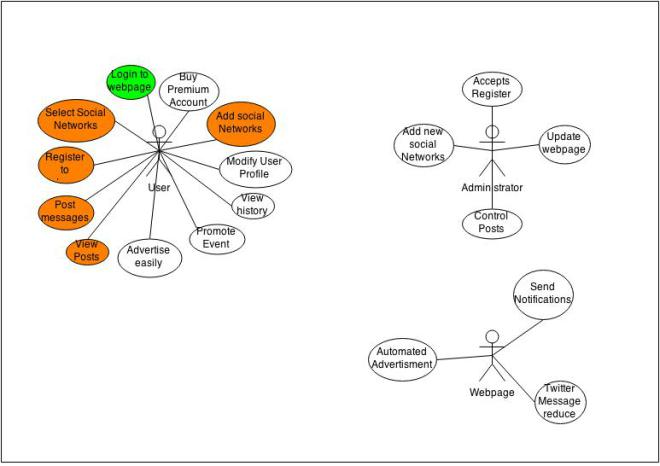
\includegraphics[width=\textwidth]{./img/usecase_socialfunnel.jpg}
\end{center}

\subsection{Product Perspective}

To be determined - Produktausblick !?

\subsection{Product Functions}

Die erste Funktion des Produkts für jeden User ist die Registrierung. Ohne einen Account anzulegen gibt
es keine Möglichkeit die Software zu benutzen, da es sich um sensible Daten handelt und Zugriff für Dritte
mit allen zur Verfügung stehenden Möglichkeiten verhindert werden soll. Dabei muss der Anwender Daten von sich selbst sowie eine gültige Mailadresse angeben.\\

Hat der Anwender ein Benutzerkonto erstellt, kann er sich auf der Webseite mit seinem Benutzernamen und 
dem dazu gehörenden Passwort einloggen. Dies führt ihn auf die individuell gestaltbare Startseite.

Um diese zu verändern kann er Accounts verschiedener Sozialer Netzwerke hinzufügen und auswählen welche
Inhalte er davon angezeigt bekommen möchte. \\

User Interaktion selbst gibt es bei Social Funnel nicht. Es wird nicht darauf abgezielt ein eigenes Netzwerk zu
erstellen, sondern lediglich bereits bestehende Plattformen sinnvoll zu bündeln. \\

Der User kann beliebig unterstütze Plattformen hinzufügen oder entfernen, dabei auch mehrere von gleichen
Anbietern. 

Der so entstandene Newsfeed kann mit Werkzeugen und Filtern auf das vom Anwender gewünschte 
Angebot zurecht geschnitten werden.

Neben dem Empfangen von Nachrichten steht dem Anwender auch die Möglichkeit zur Verfügung selbst 
neue Posts zu verfassen und diese über ein Formular in alle von ihm ausgewählten Plattformen gleichzeitig
zu veröffentlichen.

\subsection{User characteristics}
 
Nutzer der Webseite haben im Allgemeinen mindestens einen Account bei einem großen sozialen Netzwerk,
in der Regel jedoch bei mehreren wie z.B. Facebook, Twitter, Google+, Instagram, Wordpress, uvm.\\

Um die Übersicht über alle Nachrichten aus diesen Plattformen behalten zu können, müssen Personen unserer 
Zielgruppe sich über Apps oder Webseiten in jedes Netzwerk einzeln einloggen um ihre Nachrichten zu überprüfen.
Social Funnel bietet dieser Personengruppe die Möglichkeit, dies gebündelt an einer zentralen Stelle zu erledigen. 

\subsection{Constraints}

To be determined - Einschränkungen

\subsection{Assumptions and Dependencies}

\paragraph{Voraussetzungen:} Für den Gebrauch der Anwendung braucht der Nutzer einen Internetzugang, 
sowie einen Account bei einem der Sozialen Netzwerke, die eingebunden werden.
Auch muss er sich innerhalb der Webanwendung einmal in den gewünschten sozialen Netzwerken anmelden, 
um diese über den Account der Web-Anwendung nutzen zu können.\\

\paragraph{Abhängigkeiten:} Die Anwendung funktioniert nur, wenn die Zielsysteme (Sozialen Netzwerke) funktionieren. 
Sollte es auf einer der anderen Seiten Probleme geben, kann diese nicht angesprochen werden.\\

\subsection{requirements subsets}

to be determined

\section{Specific Requirements}

\subsection{Functionality}

\subsubsection{User}

\paragraph{Registrieren}

Der Benutzer soll hierbei einen Account bei Social Funnel anlegen können. Dazu soll er seinen Namen,
Geburtsdatum, ein Passwort und einen frei Wählbaren Benutzernamen angeben. Neben diesen Angaben ist noch
eine gültige Email-Adresse nötig zur Bestätigung der Registrierung und spätere Benachrichtigungen.\\
\href{https://github.com/wayoflife/softwareengineering/blob/master/Dokumentation/Use_Cases/UC_Registrieren.pdf?raw=true}{\emph{Link zur Use-Case Specification}}

\paragraph{Login}

Mit den bei der Registrierung eingegebenen Daten kann der Benutzer sich auf die Seite einloggen.
Dafür ist eine Kombination aus Mailadresse und Passwort notwendig.\\
\href{https://github.com/wayoflife/softwareengineering/blob/master/Dokumentation/Use_Cases/UC_Einloggen.pdf?raw=true}{Link zur Use-Case Specification}

\paragraph{Soziales Netzwerk hinzufügen}

Hier kann durch eine simple Eingabemaske ein unterstütztes Netzwerk ausgewählt werden
und zu den eigenen hinzugefügt werden.\\
\href{https://github.com/wayoflife/softwareengineering/raw/master/Dokumentation/Use_Cases/UC_SozialeNetzwerkehinzufuegen.pdf}{Link zur Use-Case Specification}

\paragraph{Soziales Netzwerk ändern/entfernen}

Über eine Liste können hier hinzugefügte Netzwerke verändert oder entfernt werden.\\
\href{https://github.com/wayoflife/softwareengineering/raw/master/Dokumentation/Use_Cases/UC_SozialeNetzwerkeentfernen.pdf}{Link zur Use-Case Specification}

\paragraph{Bei sozialen Netzwerk registrieren}

Mit einer unterstützenden Eingabemaske können hier von gewünschten Netzwerken die Registrierungsseiten
aufgerufen werden und im Anschluss direkt zu den eingebundenen Seiten hinzugefügt werden.

\paragraph{Nachrichten Filtern}

Mit Auswahl von erweiterbaren Filterkriterien lässt sich der persönliche Newsfeed (oder mehrere) individuell 
anpassen.

\paragraph{Nachrichten abschicken}

Es gibt eine Eingabemaske, in der Nachrichten verfasst und abgeschickt werden können.\\
\href{https://github.com/wayoflife/softwareengineering/raw/master/Dokumentation/Use_Cases/UC_NeuenPostVerfassen.pdf}{Link zur Use-Case Specification}

\paragraph{Soziale Netzwerke auswählen}

Über Checkboxen kann ausgewählt werden, in welchen Netzwerken die Nachricht veröffentlicht werden soll.

\paragraph{Userdaten verwalten}

Hier kann der Anwender seine eigenen Daten aktualisieren und verändern, wie zb eine neue Mailadresse
oder das Ändern des Passworts.

\paragraph{Premiumaccount kaufen}

Falls auf der Webseite Werbung geschaltet wird, soll es möglich sein, sich einen Premium Account zu erwerben, um keine Werbung angezeigt zu bekommen.

\paragraph{Nachrichtenverlauf ansehen}

In einer Historienseite, soll man den bisherigen Verlauf an Posts nachvollziehen können.

\paragraph{Werbung schalten}

Für Geschäftstreibende soll es möglich sein, zeitgesteuerte Werbenachrichten abzuschicken. 

\paragraph{Ereignis bewerben}

Ebenfalls soll es ermöglicht werden, Veranstaltungen über SocialFunnel zu planen und zu verteilen.

\subsubsection{Administrator}

\paragraph{Registrierungen akzeptieren}

Der Administrator soll zu Beginn noch Anmeldungen zu SocialFunnel akzeptieren und den User freischalten.

\paragraph{Neue soziale Netzwerke}

Außerdem wird es eine Möglichkeit geben, neue Soziale Netzwerke einzubinden, die für User dann freischaltbar werden.

\paragraph{Webseite updaten}

Ebenfalls muss der Administrator die gesamte Webseite updaten können.

\paragraph{Posts überwachen}

Als letzte Aufgabe müssen Stichprobenweise Posts überprüft werden, um Gesetzesverstöße (Rechtes Gedankengut, CyberMobbing, …) ausschließen zu können.

\subsubsection{Webseite}

\paragraph{Werbung schalten}

Die Webseite soll automatisch Werbung schalten, je nach User.

\paragraph{Benachrichtigungen senden}

Falls neue Nachrichten aus Netzwerken beim User eingehen, soll dieser darauf hingewiesen werden.

\paragraph{Nachrichten kürzen}

Da Twitter eine Zeichenbegrenzung hat, soll die Webseite die Länger der Nachricht für Twitter gekürzt werden.

\subsection{Usability}

\subsubsection{Benutzeroberfläche}

Diese soll möglichst einfach und schmal gehalten werden. Alle Inhalte der Webseite werden aus externen Quellen
geliefert. Die Software soll lediglich als Rahmenprogramm für diese Plattformen dienen und eine leichte
Bedienoberfläche zur Verfügung stellen. 

Dabei soll die Nutzung intuitiv sein und simple Formulare für das hinzufügen und entfernen bereitgestellt werden.
Die Auswahl für den anzuzeigenden Inhalt soll durch Checkboxen mit wenigen Clicks möglich sein und in Echtzeit
aktualisiert werden.

\subsection{Reliability}

\subsubsection{Erreichbarkeit} 

Die Webseite soll im Optimalfall eine Uptime von 24/7 vorweisen können. Ausfälle können jedoch leicht verkraftet
werden, da für den Nutzer lediglich die von Social Funnel bereitgestellt Features fehlen, er allerdings auf den
Webseiten der Netzwerke noch immer vollen Zugriff hat.

Diese Ausfälle können durch technische Störungen oder Wartungsarbeiten ausgelöst werden. In beiden
Fällen wird versucht die Dauer des Ausfalls auf ein Minimum zu reduzieren.

\subsection{Performance}

to be determined

\subsubsection{Antwortzeit}

Die Webseite soll maximal einen Ping von 500 ms unterstützen, es ist jedoch eine durchschnittliche Verbindung
von unter 100 ms anzustreben um einen flüssigen Auftritt zu garantieren.

\subsection{Supportability}

n/a

\subsection{Design Constraints}

\subsubsection{Spring}

Spring ist eine Sammlung von Bibliotheken des Spring Projekts %\cite{spring}

\subsubsection{Hibernate}

Wird verwendet als Verbindung mit der Datenbank \cite{hibernate}

\subsubsection{Vaadin}

Wird als Framework zur Erstellung der Webseite verwendet %\cite{vaadin}

\subsubsection{Git}

Wird zur Versionsverwaltung der Software sowie der Dokumentation verwendet %\cite{git}

\subsubsection{Lombok}

Wird zum Einsparen von Code verwendet \cite{lombok}

\subsubsection{Jenkins}

\cite{jenkins}

\subsubsection{Maven}

\cite{maven}

\subsection{On-line User Documentation and Help System Requirements}

Ist auf der Webseite Verfügbar in Form einer Hilfe Seite, sowie einem Service Formular
siehe Use Case Help

\subsection{Purchased Components}

n/a

\subsection{Interfaces}

\subsubsection{User Interfaces}

n/a

\subsubsection{Hardware Interfaces}

n/a

\subsubsection{Software Interfaces}

n/a

\subsubsection{Communications Interfaces}

n/a

\subsection{Licensing Requirements}

Keine Lizenzierungen notwendig. Jegliche benutzte Fremdsoftware unter der MIT Lizenz verfügbar.

\subsection{Legal, Copyright and other Notices}

Software wird unter der MIT Lizenz veröffentlicht, damit OpenSource.

\subsection{Applicable Standards}

n/a

\section{Supporting Information}

n/a

\end{document}
